% !TeX root = these.tex

\chapter{Cadre technologique}


\section{Développement du côté client}
%*****************************Google Web Toolkit***************************
\subsection{Google Web Toolkit (GWT)}

	%************************ Présentation *********************************
\subsubsection{Présentation}
GWT est un outil open source mis en ligne par Google permettant de développer des applications web avancées. En utilisant cet outil, nous pouvons développer des applications AJAX en langage Java.
Lors de l'élaboration d'une application, le cross-compiler de GWT traduit la partie cliente de l'application java en 
fichiers JS. Ces fichiers peuvent être soumis à des optimisations (obscurcir le code, séparation du JS en plusieurs 
´
% JP : J'utilise la phrase "just another librairy" Peut on laisser ça sous cette forme?
fichiers, etc.). GWT n'a pas pour objectif d'être "just another library" mais possède sa propre philosophie.\\
\newline
\indent
Pour programmer une application web de notre type, il faut maîtriser des outils comme l'AJAX\footnote{Asynchronous JavaScript And XML}, l'HTML ainsi que le CSS. Le problème principal de ces outils est la compatibilité entre les différents navigateurs. La façon de mettre en forme un site web n'aura pas toujours le même sur ceux-ci. Il faut prendre en compte aussi la complexité d'utilisation de ces langage de manière avancée (utilisation du DOM en HTML,etc.). Le langage JS est assez complexe d'utilisation, surtout pour l'écriture de grosses applications, le debuggage de celles-ci étant assez fastidieux puisqu'il s'agit d'un langage interprété.
\newline
\indent
Pour pallier à ces problèmes, GWT à été créé. Il a été élaboré dans le but de répondre à un besoin, et non pas de proposer une autre librairie standard. Il s'agit d'une vrai boite à outils, et propose des solutions de développement répondant aux besoins du programmeur.
% ici je rajouterais qq lignes sur le fait que gwt est énormément utilisé par 
% des société prestigieuse ainsi que google
\newline
\indent
GWT est utilisé par exemple dans des outils web de Google comme Gmail. Nous pouvons aussi citer l'entreprise Rovio à l'orignie du jeux a succès Angry Bird ayant développer une version HTML5 du jeux à l'aide de GWT\footnote{cf. https://developers.google.com/web-toolkit/casestudies/}.

%************************ Principe de fonctionnement *********************************
\subsubsection{Principe de fonctionnement}
GWT possède un plugin Eclipse (et pour d'autre IDE\footnote{Integrated Development Environment} comme NetBeans, JDeveloper, etc.), Eclipse étant l'IDE que nous avons choisi. Ce plugin, dans sa version Eclipse, permet d'intégrer les outils GWT à l'IDE et de faciliter son utilisation pour l'utilisateur en automatisant par exemple, la structure des différents packages java.
\newline
\indent
Comme nous l'avons expliqué précédemment, le principe de fonctionnement de GWT est de pouvoir créer des applications web basé en langage Java, sur un modèle client/serveur, et de convertir la partie cliente de l'application en JS, la partie serveur restant elle, en java. Un autre aspect de se fonctionnement réside dans la compilation pouvant être éffectuée pour un ou plusieurs navigateurs spécifique, favorisant la compatibilité et l'homogénéité du logiciel sur chacun d'entre eux. Ces deniers chargent uniquement ce qui les concernes. En plus de ces différents aspects qu'offre GWT, il permet aussi de préciser quelles sources du code\footnote{correspondant au .CLASS généré lors de l'exécution du code java} prendre en compte pour un navigateur spécifique.

%************************ Mode de fonctionnement *********************************
\subsubsection{Mode de fonctionnement}
Nous distinguons deux types de fonctionnement. Le mode de développement ainsi que le mode de production.
	
\paragraph{Mode de développement}
Le mode de développement consiste à compiler les sources du projet. Celui-ci n'est pas retranscrit en JS mais est directement exécuté en byte code. Ceci afin de permettre le debuggage de l'application. GWT compile tout de même le projet en JS-HTML-CSS afin de pouvoir valider le projet.
Pour pouvoir utiliser le mode de développement, il est nécessaire d'installer au préalable le plugin de développement sur le navigateur web. Ce plugin permet de capturer les événements et actions venant du client pour ensuite les envoyer vers le serveur local lancé au moment de l'exécution du projet.
\paragraph{Mode de production}
Le mode de production correspond au code JS généré par le compilateur GWT. Le compilateur créer le JS, HTML et CSS a partir de sources du projet. Ce code correspond à l'application final qui pourra être déployer sur notre serveur Tomcat.

%****************************Architecture de GWT******************************
\subsubsection{Architecture GWT}
L'architecture d'un projet GWT se fait sous la forme de client/serveur. Nous allons analyser comment ce déroule la communication entre ces deux parties. Nous distinguons deux types de communication dans l'application.
\begin{itemize}
\item Client/Client: communication entre les différentes vue de l'application
\item Client/Serveur: utilisant le protocole RPC\footnote{Remote Procedure Call} 
\end{itemize}
\paragraph{Évènement}
Afin de pouvoir gérer la communication entre les différentes vues de l'application, GWT utilise un système d'envoi d'évènements (appelé Events). Ceux-ci permetent aux vues de dialoguer entre elle.
Par exemple, une application GWT peu posséder une en-tête. Celle-ci est statique et n'est pas recharger entre les différentes vues. Lors de l'identification, les informations de connexion peuvent être envoyées à la vue suivante pour spécifier à l'utilisateur le nom du compte sur lequel il est connecté.
Les events sont enregistré auprès de l'eventbus. Cet eventbus peut être écouté pour récupéré les informations voulues.

\paragraph{Actions}
Les actions ressemble au Event, à l'exception que celles-ci sont envoyées au serveur. Elle permette par exemple de faire des requêtes vers la base de données pour recueillir certaines informations. Pour rester dans le même exemple, lorsqu'un utilisateur se connecte à l'application en spécifiant sont identifiant et son mot de passe, ceux-ci doivent être vérifié dans la base de données qui va renvoyer, dans le cas ou l'utilisateur existe, la liste des projets qui lui sont assignés. Cette méthode ce fait à l'aide du protocole JSON\footnote{JavaScript Object Notation}/RPC. Les appels se font de manière asynchrone permettant de ne pas bloquer le client lors d'un appel de procédure.
	
%***************************** Avantage de GWT****************************
\subsubsection{Avantages}

\paragraph{Facilité d'utilisation}
Le premier avantage que nous citerons est la facilité d'installation et d'utilisation de l'outil. Pas besoin de configuration fastidieuse. Installer l'IDE, Installer le Plugin, et ça fonctionne.
La possibilité de pouvoir coder sont application à l'aide d'un langage de haut niveau facilite le développement.

\paragraph{Debbugage}
Il permet un debuggage rapide du code, celui-ci étant codé en java et non pas en JS qui est un langage interprété.

\paragraph{Optimisation}
Optimisation du code, obfuscation de celui-ci, compression du JS, mise en cache, séparation du JS en différent fichier, etc.

\paragraph{prédéfini de composant}
Différent widget prédéfini sont disponible, ainsi, pas besoin de codage fastidieux dans le designer d'un bouton, une boite de dialogue, etc. avec la possibilité de créer ses propres widget.

\paragraph{Code adapter en fonction du navigateur}
Le code java est traduit en code JS et automatiquement adapté au navigateur de notre choix.

\paragraph{JSNI (JavaScript Native Interface)}
GWT offre la possibilité d'utiliser directement du code JS au sein même de notre application. Il est donc tout à fait possible d'utiliser des librairies externes entièrement codée en JS comme Jquery.

\paragraph{Utilisation de GinJector et Guice}
GinJector n'étant pas un principe propre GWT permet de créer une indépendance entre les différentes classes du projet. Ainsi, si nous voulons utiliser une object ou une classe dans une autre, il n' y a pas besoin d'instancier cette nouvelle classe. Nous pouvons simplement injecter.

%**************************** Inconvénient de GWT **************************************
\subsubsection{Inconvénients}
Le principal inconvénient que nous avons pu noter suite à notre expérience personnelle est lorsque l'application atteint un état d'avancement plus avancé, il devient très lourd et très lent de tester son application en mode développement. La JVM\footnote{Java Virtual Machin} devant traduire le code est très lente. Il nous a fallu en moyenne 5 minutes pour charger une page, et nous avons eu frequement des erreurs de type "out of memory" du à la lourdeur de la tache effectuer par l'ordinateur. Pour certains types de test, nous nous somme retrouver dans l'obligation de déployer l'application sur notre serveur tomcat, car la traduction du java vers le JS étant très lourde, certaines partie devait être tester directement en mode production (notamment le drag and drop,…). De même, lorsque l'application doit charger une grande quantité d'information (grand nombre de cartons, professeurs,…) la page mais beaucoup de temps à s'ouvrir.\\
Autre inconvénient, le temps de compilation du logiciel. Celui-ci peut être très fastidieux en fonction des paramètres demandé.
	
Un autre inconvénient est la limitation des widgets fournis de base dans l'application. Pour certaines chose plus avancée nous avons du avoir recourt à des librairie externe, bien que celle-ci ne soit pas aussi performante (comboBox avec CheckBox,…).

%************************* GWT DESIGNER *******************************
\subsection{GWT-Designer}
GWT-Designer est un outils permettant de créer de manière simple les interfaces graphiques. Celle-ci est crée via un fichier XML\footnote{eXtensible Markup Language} et est retranscrite en code java par le compilateur. Ce code XML est éditable "manuellement" ou peut être créer à l'aide d'une interface de drag and drop ou les composants (widgets) peuvent être sélectionné. L'avantage d'utiliser un tel outil est la bonne pratique que celui-ci apporte, permettant de faire une distinction entre les différentes partie du code.

%************************* GWT PLATEFORM *********************************$
\subsection{GWT - Plateform}

\subsubsection{Présentation}

GWT plateform est un framework basé sur le MVP\footnote{Model View Presenter} et permettant de mieux structurer notre projet en respectant une certaine méthode. Ce framework s'incorpore directement à l'IDE et est dépendant de GWT.
	
\subsubsection{Le model View Presenter}
Le MVP se base sur le MVC\footnote{Model View Controler}. Celui-ci est un design pattern fournissant une manière d'élaborer des interfaces graphique. Il est séparé en trois partie, le modèle de données, les différentes vues de l'application (L'interface du client) et le présenteur (correspondant au controleur du MVC). La partie intéressante de ces modèles réside dans l'utilisation d'un controleur/présenteur, ou transite les informations. L'application est soumise à leur contrôle ce qui permet d'avoir une application plus solide. Dans le MVC le contrôleur s'occupe de gérer les évènements. La logique de contenu (Rendering logic) se passe directement entre le modèle et la vue. En MVP, cette logique est gérée par le présenteur. Plus rien ne transite directement entre l'interface et le modèle mais est soumise au contrôle du présenteur.

%*************************** LIBRAIRIE EXTERNE GWT **************************
\subsection{Libraire externe}
Pour la création d'une interface plus avancée nous avons du nous diriger vers des librairies externes. 
\subsubsection{GWT-DND}
Nous avons utilisé GWT-dnd qui comme son nom l'indique nous a permis
d'implémenter le drag and drop sur les cartons. Le drag and drop fournis par
cette librairie nous permet de capturer les EVENTS de la souris mais aussi les EVENTS touch permettant de garder la possibilité qu'offre GWT d'être utilisé sur des appareils mobiles. Ce qui est non négligeable à l'heure actuelle ou les smartphones et tablettes on une place prépondérante sur le marché. Cette librairie permet de rendre dragable n'importe quel widget ou un ensemble de ceux-ci.
\newline
\indent
L'outil est simple d'utilisation. Pour pouvoir rendre dragable notre widget, il est nécessaire de créer un "dragControler". Les widgets s'enregistre auprès de ce contrôleur. Une fois cette opération effectuée, il faut pouvoir définir une zone ou ces widgets pourons être droper. Pour ce faire, nous créons un nouveau "dropControler", celui-ci s'enregistre aussi auprès du dragControler pour signifier qu'il est près à recevoir les widgets.

\subsubsection{Smart-GWT}
Smart-GWT est un wrapper\footnote{Un adaptateur} de la librairie JS SmartClient. Elle propose un grand nombres de widget venant s'ajouter à ceux fournis par GWT. Puisque Smart-GWT n'est qu'un wrapper de la smartClient, elle ne respecte pas l'idée de base de GWT voulant que le code soit écrit totalement en java et ensuite traduit en JS. Nous avons pu noter que les widgets proposé par cette librairie ne sont pas aussi réactif que ceux de GWT.
\newline
\indent
Ces deux libraires ont été spécialement conçue pour être utilisée avec GWT. Il ne s'agit pas de librairie JS comme Jquery, mais bien de librairie\footnote{Fournies sous la forme de .JAR} orienté GWT. Afin de pouvoir utiliser celle-ci, il est nécessaire de modifier le fichier de configuration du projet en y ajoutant les informations relatives au librairie.


%\subsection{Serveur Linux}
%SERVEUR LINUX (Debian 64bits)
%Afin de pouvoir tester notre application, nous disposons d'un serveur tomcat tournant sur une machine %linux. L'application (sous forme de ".WAR" (en comparaison au ".jar", le "W" signifiant web)) est %l'application final possédant le code javascript (et non plus du code java comme en mode de %développement).

\subsection{Les langages web}
L'évolution des navigateurs, des langages web et des possibilités que ceux-ci permettent, l'évolution de la société visant à s'orienter de plus en plus vers le cloud computing, nous montre l'utilité d'utiliser ces langages dans leurs dernières normes. Afin de proposer une application web interactive, nous nous sommes orienté sur ces derniers langages web, même si nous n'utilisons pas tout l'étendu de ce qu'ils proposent.

\subsubsection{HTML5}
GWT nous permet l'utilisation du HTML5. l'arrivée du HTML5 permet d'accroitre les performances d'une application web, en proposant des fonctionnalités plus avancées telles que l'utilisation de canvas, de balise audio ou video. Une autre fonctionnalité est l'utilisation d'un local storage, permettant de stocker une grande quantité de données.
\subsubsection{CSS3}
Le design général de l'application a été basé sur cette dernière norme. Il est donc nécessaire d'avoir un navigateur à jour pour pouvoir profiter de l'avantage qu'offre cette norme.

\subsubsection{JS}
Même si le code JS est généré par le compilateur de GWT, elle est un élément essentiel de l'application. 
 
\subsection{Local Storage (LS)}
L'apparition du local storage avec le HTML5 ouvre une porte en plus au développeur d'application web. Ce dernier permet de stocker une grande quantité de données coté client. Pour bien comprendre le choix de l'utilisation de cette technologie, nous allons le comparer avec le cookie.

\subsubsection{Local Storage vs Cookies}


\begin{tabular}{|l|c|c|}
  	\hline
   		& Local Storage & Cookie \\
  	\hline
  		Stockage: & 5MB & 80KB (4KB/cookie, 20cookies/domaine) \\
	\hline  
  		Utilisation de la B.P.: & Aucune & Envoi des données à chaque requête vers le domaine \\
  	\hline
  		Performance: & Data mise en cache du navigateur & Data envoyé répétitivement vers le domaine \\
  	\hline
  		Contraintes: & aucune & 300 cookies maximum \\
  	\hline
  		Rapidité: & très rapide (données chargé en cache au démarrage & plus lente (serveur vérifie si le cookie existe) \\
  	\hline
\end{tabular}
%LOCAL STORAGE
%Capacité de stockage : 5MB
%Utilisation de la bande passante: Aucune, tout est stocker chez le client)
%Performance: Data mise en cache du navigateur
%contraintes: aucune
%rapidité: rapide (charge les données de la cache au démarrage)

%COOKIE
%Capacité de stockage: 80KB (4KB/cookie 20cookies/domaine)
%Utilisation de la BP: Envoi des données a chaque requete vers le domaine
%Performance: Data envoyé répétitivement vers le domaine
%contraintes: 300 cookies maximum
%rapidité: plus lente (serveur vérifie si le cookie existe)

Tout comme les cookies, les informations contenu dans le local storage ne peuvent pas contenir d'informations sensibles\footnote{Comme les numéros de carte de crédit}. Nous ne nous sommes pas attardé sur ce point car les informations contenu dans notre local storage ne sont pas utile pour les Hackers, inutile donc de crypter le nom d'un professeur. 

L'utilisation du local storage permet, comme les cookies, de partager les données entre les différents onglets du navigateur. Nous aurions pu nous orienter vers une solution plus simple, comme enregistrer les informations de la partie cliente dans des tableaux ou listes, mais les informations ne seraient plus partager entre les onglets et fenêtres du navigateur, ce qui limiterait de manière drastique l'utilisation du programme. Le local storage à donc bon nombres d'avantages et l'utilisation et la mise en place de celui-ci, bien qu'étant une partie fastidieuse, était pour nous nécessaire au bon développement de l'application ainsi qu'à son développement futur.

\subsubsection{Principe}
Le principe de ce local storage est donc de fournir un moyen de stocker et d'accéder rapidement aux données tout en limitant le trafic entre le client et le serveur. Nous ne rentrerons pas dans la structure de celui-ci, ce point faisant partie d'un autre chapitre. Les informations sont mise en cache et peuvent être supprimées à tout moment par l'utilisateur.
\subsubsection{Utilisation dans notre application}
Lors de chaque modifications (comme le placement d'un carton), nous enregistrons ces changements dans le local storage ainsi que dans la base de données de manière asynchrone afin de permettre une grande rapidité de l'application. Dans l'hypothèse ou la base de données ne serait plus accessible (ex: perte de connexion) nous avons implémenté une fonctionnalité\footnote{version alpha} permettant de synchroniser l'état du local storage avec la base de données lors d'un retour de connexion.\\
\\
Actuellement, une connexion internet est requise lors d'un rechargement de la page afin de se mettre à jour, ceci est indispensable pour offrir une synchronisation cohérente. Cependant une fonctionnalité, en Alpha actuellement, permet, si l'option est activé ou si la bdd n'est pas accessible, de fonctionner sans cette dernière, et lors de la récupération de la connexion, les données sont alors synchronisé.



\section{Développement du côté serveur}

\subsection{Java EE}

% A retravailler
La plateforme Java entreprise édition est un ensemble de spécifications portées par un consortium de sociétés internationales qui offrent, ensemble, des solutions pour le développement, le déploiement et la gestion des applications d'entreprises multi-niveaux, basées sur des composants.

\begin{figure}[!h]
    \center
   	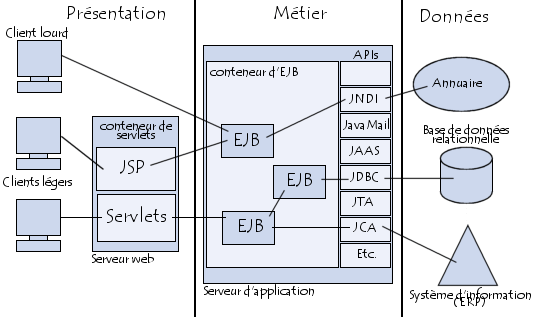
\includegraphics[scale=0.65]{architecture_JEE.png}
   	\caption{Diagramme issu de\url{architecture_JEE.png}}
    \label{reference1}
\end{figure}

Et dans la figure  \ref{reference1}\footnote{Diagramme issu de \url{}}
** image**
Construit sur la plateforme de Java 2 édition standard (Java SE), la plateforme Java EE ajoute certaines fonctionnalités nécessaires pour fournir une plateforme complète, stable, sécurisée et rapide de Java au niveau entreprise. 
Dans la mesure où J2EE s'appuie entièrement sur le Java, il bénéficie des avantages et inconvénients de ce langage, en particulier une bonne portabilité et une maintenabilité du code.\\
\newline
\indent
L'ensemble de l'infrastructure d'execution JavaEE est donc constitué de services (API) et spécifications tel que:
\begin{itemize}
\item HTTP et HTTPS
\item Java Transaction API (JTA)
\item Remote Method Invocation/Internet Inter-ORB Protocol (RMI/IIOP)
\item Java Interface Definition Language (Java IDL)
\item Java DataBase Connectivity (JDBC)
\item Java Message Service (JMS)
\item Java Naming and Directory Interface (JNDI)
\item API JavaMail et JAF (JavaBeans Activation Framework)
\item Java API for XML Processing (JAXP)
\item Java EE Connector Architecture
\item Gestionnaires de ressources
\item Entreprise Java Beans (EJB)
\item Java Server Pages (JSP)
\item Servlet
\item Java API for XML Web Services (JAX-WS, anciennement JAX-RPC)
\item SOAP with Attachments API for Java (SAAJ)
\item Java API for XML Registries (JAXR)
\end{itemize}
Dans le cadre de notre application, seule une sous partie de ces composants on été utilisé, tel que les servelets, les JSP, JavaMail ou encore JDBC avec Hibernate, tel que décrit dans le point suivant.

De plus, l'architecture J2EE repose sur des composants distincts, interchangeables et distribués, ce qui signifie notamment :
\begin{itemize}
\item qu'il est simple d'étendre l'architecture 
\item qu'un système reposant sur J2EE peut posséder des mécanismes de haute-disponibilité, afin de garantir une bonne qualité de service ;
\item que la maintenabilité des applications est facilitée.
\end{itemize}

% === avantages
Ces outils favorisent l'interaction avec, d'une part, le solveur, et d'autre part, la base de données. Cela constitue un avantage majeur de notre application. Java EE regroupe donc nativement ces libraires dans un endroit unique. Il n'est plus utile de chercher un framework adapté à nos besoin et de devoir faire face à des implémentations, parfois fastidieuse, de ce dit framework, augmentent par ce fait la cohérence du programme et favorisant la maintenance de celui-ci. Ce type de choix favorise le debuggage de l'application.

%% === apprentissage
Bien qu'ayant déjà utilisé et programmé en Java SE, nous ne nous étions jamais retrouver confronté au Java Entreprise Edition. La différence entre ceux - ci se trouve surtout dans la complexité de leur utilisation. Le java SE ayant une approche plus orienté desktop, le Java EE proposant des outils avancés permettant de faire des applications internet (notamment web, mail, etc.), nécéssitant un temps d'apprentissage et d'adaptation. Utiliser du Java EE nous a permis d'en apprendre plus sur ce langage fort demandé en entreprise. Connaitre ce langage constitue un atout majeur pour un développeur, nous sommes ravis d'avoir pu utiliser une partie des possibilités offert par ce langage couplé au outils java EE .

Pour le log des données coté serveur, nous avons également utilisé log4j qui nous à permis de faciliter le travail de debuggage l'application.

\subsection{Hibernate}

Pour pouvoir communiquer avec notre base de données à partir de notre code java, nous avons tout d'abord utilisé JDBC. Nous avons ensuite choisi d'utiliser Hibernate, étant une couche supérieure à JDBC. Hibernate permettant de pouvoir transformer les tables en object, celui-ci offre une bonne cohérence avec l'application.

Hibernate est un framework libre, appellé framework de  \enquote{mapping objet-relationnel} ou encore de \enquote{persistance objet des données} (voir Figure \ref{reference2}). 
\begin{figure}[!h]
    \center
   	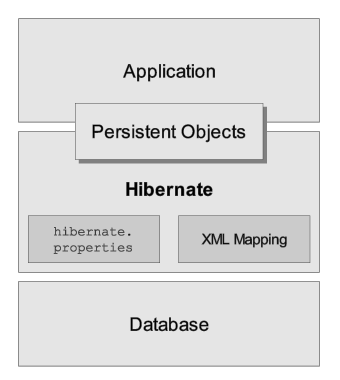
\includegraphics[scale=0.65]{schema_hibernate.png}
   	\caption{Diagramme issu de\url{}}
    \label{reference2}
\end{figure}
Cela permet donc à la couche applicative de notre programme de traiter les données venant de la base de données comme des objets, fournissant un mapping entre le relationelle et l'orienté objet. La base de données peut être traité aves les avantages de l'orienté object (comme le polymorphisme, l'héritage, etc.). Le lien entre les classes exposées et la source physique des données  est définie par un fichier xml d'où le mapping objet-relationnel.
Cela nous à donc permit de gérer notre base de données, comme le reste de l'application en orienté objet, et même si son apprentissage ne fut pas des plus aisée, la gestion générale du code s'en est retrouvé grandement amélioré.

Un autre avantage recherché par cette solution, est que son indépendance à la base de donnée le entièrement portable, et, sans aucune modification du code, nous rappelons que notre application peu tourner sur 221 base de données différentes.  Notre application, après avoir configuré ses crédential dans le fichier de configuration d'Hibernate, se chargera de créer l'entièretée des tables et la structure de la base de donnée.

Théoriquement il aurait donc été possible d'envoyer directement un objet "hibernate" (représentant par exemple une table de notre base de données), à GWT, donc à l'utilisateu. malheureusement la théorie n'est pas toujours applicable, et comme stipulé dans la doc GWT\footnote{https://developers.google.com/web-toolkit/articles/using\_gwt\_with\_hibernate},
une SerializationException est levée à chaque fois qu'un type transférée via RPC n'est pas «sérialisable». La définition de la sérialisibilité signifie ici que le mécanisme RPC - GWT sait comment sérialiser et désérialiser le type de bytecode au format JSON et vice-versa.
Le problème vient du fait qu'Hibernate modifie les objets afin de les rendre persistant\footnote{pour être exact, c'est la librairie javassist qui se charge de réécrire le bytecode de ces objects pour les rendre persistant}. Au moment du transfert de l'objet, une serialisation est tantée, mais l'objet n'étant pas le même (car modifé par javassist), il ne peut être sérialisé par RPC-GWTP.
Il a fallut donc rajouter des classes de type DTO\footnote{Data Transfer Object}, qui, étant sérialisable, ont pu servir de communication entre la partie cliente et serveur.

Hibernate possedant sont propre language de requète HQL \footnote{Hibernate Query Language}, d'apparence similaire au SQL, mais pleinement orienté Object et comprenant des notions comme l'inheritance ou le polymorphisme\footnote{https://docs.jboss.org/hibernate/orm/3.3/reference/en/html/queryhql.html}. Nous n'avons pas pu tirer pleinement avantages et n'étant pas habituer à ce genre de pratique, il a été parfois déroutant d'utiliser un langage mélangeant le SQL et les notions d'orienté objet.

